   
\documentclass[11pt]{article}
\renewcommand{\baselinestretch}{1.05}
\usepackage{amsmath,amsthm,verbatim,amssymb,amsfonts,amscd, graphicx}
\usepackage{graphics}
\topmargin0.0cm
\headheight0.0cm
\headsep0.0cm
\oddsidemargin0.0cm
\textheight23.0cm
\textwidth16.5cm
\footskip1.0cm
\theoremstyle{plain}
\newtheorem{theorem}{Theorem}
\newtheorem{corollary}{Corollary}
\newtheorem{lemma}{Lemma}
\newtheorem{proposition}{Proposition}
\newtheorem*{surfacecor}{Corollary 1}
\newtheorem{conjecture}{Conjecture} 
\newtheorem{question}{Question} 
\theoremstyle{definition}
\newtheorem{definition}{Definition}

\begin{document}
\title{Trigonometry}
\author{Cameron Dart}
\maketitle

\section{Background Info}

This documented is aimed to give an introduction to trigonometry.

\subsection{Angles}
An angle, denoted $\theta$ or $\beta$, is how we measure the distance between two lines or planes.\\
Sin, Cosine? Tangent?
\subsection{How Do We Measure Angles?}\label{section:mathmode}

\subsection{Some Old Hippie Caught Another Hippie Tripping On Acid}\label{section:mathmode}
Didn't expect that now did you?  Now that you read that I'm sure you'll never forget what SOA CAH TOA is how we remember our trigonometric functions.\\
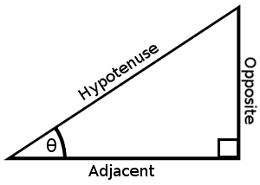
\includegraphics[scale=0.5]{img/triangle.png}
\subsection{Useful Theorems}
\begin{theorem}
	$sin(\theta) = \frac{opposite}{hypotenuse}$
\end{theorem}
\begin{theorem}
	$cos(\theta) = \frac{adjacent}{hypotenuse}$
\end{theorem}
\begin{theorem}
	$tan(\theta) = \frac{opposite}{adjacent}$
\end{theorem}
\begin{theorem}
	$csc(\theta) = \frac{hypotenuse}{opponent}$
\end{theorem}
\begin{theorem}
	$sec(\theta) = \frac{hypotenuse}{adjacent}$
\end{theorem}
\begin{theorem}
	$cot(\theta) = \frac{adjacent}{opposite}$
\end{theorem} 
\begin{theorem}
	$cot(\theta) = \frac{adjacent}{opposite}$
\end{theorem}

\end{document}